% ------------------------------------------------------------------------------
% LaTeX Template: Titlepage
% This is a title page template which be used for both articles and reports.
%
% Copyright: http://www.howtotex.com/
% Date: April 2011
% ------------------------------------------------------------------------------

% -------------------------------------------------------------------------------
% Preamble
% -------------------------------------------------------------------------------
\documentclass[abstract=on,paper=a4, fontsize=12pt]{scrartcl}		% KOMA article

\usepackage[a4paper,pdftex]{geometry}										% A4paper margins

\usepackage[english]{babel}
\usepackage[protrusion=true,expansion=true]{microtype}	
\usepackage{amsmath,amsfonts,amsthm,amssymb}
\usepackage{graphicx}
\usepackage{hyperref}

% ------------------------------------------------------------------------------
% Definitions (do not change this)
% ------------------------------------------------------------------------------
\newcommand{\HRule}[1]{\rule{\linewidth}{#1}} 	% Horizontal rule

\makeatletter							% Title
\def\printtitle{%						
    {\centering \@title\par}}
\makeatother									

\makeatletter							% Author
\def\printauthor{%					
    {\centering \large \@author}}				
\makeatother							
\hypersetup{}
\setkomafont{disposition}{\normalfont \bfseries}
% ------------------------------------------------------------------------------
% Metadata (Change this)
% ------------------------------------------------------------------------------
\title{	\normalsize \textsc{Senior Design} 	% Subtitle of the document
		 	\\[2.0cm]													% 2cm spacing
			\HRule{0.5pt} \\										% Upper rule
			\LARGE \textbf{\uppercase{Cost-Efficient Analysis \& Generation of Polyphonic Music}}	% Title
			\HRule{2pt} \\ [0.5cm]								% Lower rule + 0.5cm spacing
			\normalsize \today									% Todays date
		}

\author{
		Matt Bagnara\\	
		Purdue University\\	
		ECET Department\\
    West Lafayette, Ind.\\
        \texttt{mbagnara@purdue.edu} \\
}


\begin{document}
% ------------------------------------------------------------------------------
% Maketitle
% ------------------------------------------------------------------------------
\begin{titlepage}
\thispagestyle{empty}				% Remove page numbering on this page

\printtitle									% Print the title data as defined above
  	\vfill
\printauthor								% Print the author data as defined above
    \vfill
    Signed: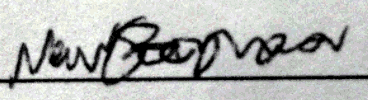
\includegraphics[height=1cm]{img/signature.png}\\
    This document may not be reproduced by any means without written consent of the author.
\end{titlepage}
\newpage
% ------------------------------------------------------------------------------
% Begin document
% ------------------------------------------------------------------------------
\abstract{
The objective of this project is to design and construct a polyphonic digital synthesizer. A Successful synthesizer will require a well-constructed input device and a microcontroller or processing platform. The synthesizer shall incorporate pulse, triangle, and noise tracks, as well as a means of mixing/synthesis. Envelopes are anticipated, as they would allow much more musicality in dynamics. Financially, the construction of the synthesizer is to remain within a set budget. Optimally, the synth will be able to play music in real-time by the user and read data from a memory A modest key entry device shall be constructed for the user to interact with the hardware directly. The synthesizer should also include the ability to configure \& display the interaction to the user in some kind of GUI. The intent of this project is to construct a synthesizer that could be used by hobbyist and beginners alike. This would require an interface with enough usability for both amateurs and hobbyists.}
\newpage
\begin{tableofcontents}
\end{tableofcontents}
\newpage

\section{Introduction}
  \subsection{Needs}
    \par Electronic synthesizers are internationally found as means of communicating creative musical content. Chiptune is an an application of electronic synthesizers that emulate the classic 8-bit or early electronic music using the limited hardware of the time. While the ability to interpret sound data directly to a synthesizer is not new, the investigation of such a project would be an enjoyable learning experience, and perhaps create a new approach to an existing product. The design and customization can be tailored to a specific usage. Also, the usage of limited hardware is anticipated to cost less.

    \par A typical synthesizer is capable of real-time synthesis \& playback. Songs are likely stored in a removable media which can be swapped for recording. The sound emitted from a typical polyphonic electronic synthesizer is in the form of arbitrary waveforms, including a noise track for percussion.
    Synthesizer kits are also available to be built and operate. The user may prefer to purchase a commercial available option, However, a custom-made synthesizer will offer all the ability of hardware chiptune creation with the functions of a modern synthesizer at a modest price preferrable under USD\$200. 
  \subsection{Objectives}
    \par The objective of this project is to design and construct a polyphonic digital synthesizer. A Successful synthesizer will require a well-constructed input device and a microcontroller or processing platform. The synthesizer shall incorporate pulse, triangle, and noise tracks, as well as a means of mixing/synthesis. Envelopes are anticipated, as they would allow much more musicality in dynamics. Financially, the construction of the synthesizer is to remain within a set budget. Optimally, the synth will be able to play music in real-time by the user and read data from a memory A modest key entry device shall be constructed for the user to interact with the hardware directly. The synthesizer should also include the ability to configure \& display the interaction to the user in some kind of GUI. The intent of this project is to construct a synthesizer that could be used by hobbyist and beginners alike. This would require an interface with enough usability for both amateurs and hobbyists.
\section{System Overview}
    The main idea is to create a synthesizer that can interface the user through a keyboard or other key entry device. The input shall allow the instrument to be played in real-time. The user interface or display can be navigated to select different sounds or waveforms(instruments/voices) in this mode. The secondary mode allows the playback of external music data which can be connected to a workstation computer to play data. The user display would be utilized in this mode to select the music data or file to be played. The output audio would be a consumer audio interface which can be later amplified or connected to a speaker.
  \subsection{System Requirements}
    \begin{enumerate}
      \item The cost shall stay within the project budget.
      \item The synthesizer shall contain an intuitive interface for amateurs and hobbyists.
      \item The synthesizer should provide playback of recorded digital data.
      \item The synthesizer should provide real-time playtime of data.
      \item The synthesizer should synthesize digital data as polyphonic music.
    \end{enumerate}
    \subsubsection{Marketing Requirements}
      \begin{tabular}{|p{2.0cm}|p{4cm}|p{6cm}|}
          \hline
        Marketing Requirement & Engineering Requirement & Justification \\
          \hline
        1. & The budget for the synthesizer will be USD\$200, but the total cost shall not exceed USD\$225. & The budget constraint will provide a modest price.\\
          \hline
        2. & The synthesizer shall offer a visual user interface. & To provide an easy, intuitive, powerful control interface.\\
          \hline
        2. & The synthesizer will not contain more than three sublevels of menus. & Simple, easy to use interfaces that are organized will be logical to follow.\\
          \hline
        3. & The synthesizer will provide interpretation of a digital format for playback. & Playback of recorded data will require an abstraction of  music into a data representation.\\
          \hline
        4. & The synthesizer will offer a method for external storage. & External storage may easily be interfaced by a PC system for generating digital data for playback.\\
          \hline
        5. & The synthesizer will offer interface that will facilitate playing as an instrument with a response time less than 5ms. & Realtime playback will require a method the user can play the instrument.\\
          \hline
        6. & The total output frequency response should be between 30 and 12KHz. & Audio playback shall play within the average response of the human ear.\\
          \hline
        7. & The synthesizer generate no less than three voices, including one distinct square, triangle, and noise voice. & Music composed of individual waveforms can be mixed to represent a wide variety of polyphonic music.\\
          \hline
      \end{tabular}
    \subsubsection{Requirement Specification}
  \subsection{Concept Generation \& Evaluation}  
    \subsubsection{Concept Generation Tree}
      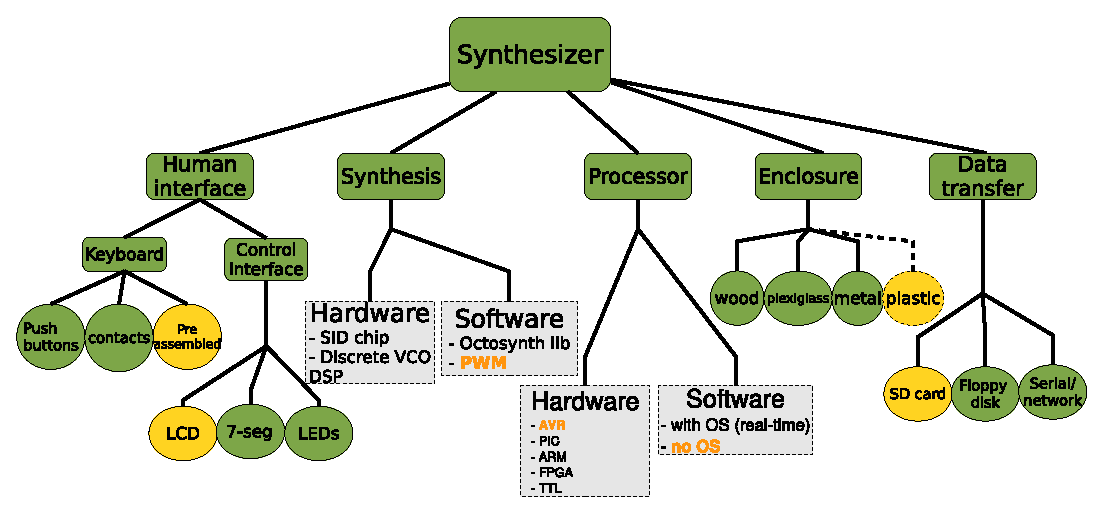
\includegraphics[width=\textwidth]{img/fig_concepttree}
    \subsubsection{Concept Blocks}
    \subsubsection{Decision Matrix}
  \subsection{System Decomposition}
    \subsubsection{Functional Decomposition}
  \subsection{Developmental Plan}
\section{Subsystem Technical Descriptions}
  Much of the testing being done will feature the debug menu which will be incorporated into the development board. The debug menu will feature self-tests documented in  Appendix J – Testing Documentation to use to verify functionality of the peripherals. The tests will run using an external serial interface on the processor and can be accessed using a serial terminal.\par
  \subsection{Synthesis subsystem}
    The Synthesis subsystem consists of the software \& hardware which creates the output waveform from the digital data being created by the processor. This subsystem is composed of software routines that create a audio buffer to write out to the DAC as well as the routines for mixing the seperate buffers. This subsystem is vital to the tonal generation of music. First of all, to verify the proper operation of the synthesis portion, the waveshape, frequencies, mixing, and other parameters need to be validated. The procedure being followed in Appendix J – Testing Documentation creates the test environment that can be used to capture the output waveform. This test environment will consist of a software debug menu, and a test board for interconnects.\par
      Synthesis is being done in both hardware and software, so both components are required. To ensure proper generation of arbitrary waveforms, the output of the synthesizer shall be connected to a 50 ohm terminated oscilloscope. The visual oscilloscope tube can be used to capture the correct waveshape for each voice. Next, the frequency range of the synthesizer will be tested using the built-in sweep function in the debug menu. The oscilloscope can, again, be used to capture the frequency vs. time data to verify this part. The voltage levels of the waveforms can also be checked at this point. The final task to verify would be the mixing capability of the synthesizer by generating polyphonic tones in the form of two, and three note chords. This may be verified by viewing a frequency-domain plot on the oscilloscope.\par
  \subsection{LCD display subsystem}
    The LCD unit consists of the LCD display, as well as the display driver being written on the software. The LCD subsystem will act as the user's interface to the synthesizer when it is being run in real-time for playback or for playback of premade audio. The purpose of this display is to provide the user with an interface. To verify the proper functionality of the display, the display of charcters, and control characters must be demonstrated. The procedure being followed in Appendix J – Testing Documentation creates the test environment that can be used to verify the display. This test environment will also consist of the software debug menu, as well as a board for connecting to the display.\par
      The LCD will operate using a user-created driver and the output shall be connected using a parallel interface. First, the verification of the display of characters will simply be done by cycling through printable ASCII characters. This will be done using the functionality of the debug menu. Also, the processing of control characters and clearing the screen will be demonstrated using this same debug screen.\par
  \subsection{PS/2 Keyboard subsystem}
    The keyboard unit consists of the PS/2 display, as well as the PS/2 driver running in software. This subsystem is used to provide key entry to the synthesizer block. It is vital to the synthesizer as it provides the only keyed input from the user. It will be used as the musicical keyboard, as well as the controls to the user-interface on the LCD. To verify the proper functionality of the keyboard, the serial communication, key press, and key release events must be demonstrated. The procedure being followed in Appendix J – Testing Documentation creates the test environment that can be used to verify the keyboard. This test environment will also require use of the software debug menu, as well as a board for connecting to the keyboard.\par
      The primary means of testing the PS/2 keyboard could be by verifying functionality on a workstation system supporting PS/2 connectivity. The application to the synthesizer will require connection to the PS/2 port on the test board. The first test will verify response of key press events by documenting the events for each key via external serial interface.  The second test will verify response of key release events by documenting the events for each key via external serial interface.\par
  \subsection{Processor subsystem}
    The processor platform subsystem consists of the microprocessor platform being used, as well as the software layer being run on it. This subsystem is the heart of the synthesizer platform, as it interfaces with all peripherals, and all software will be written on. To verify the proper functionality of the processor, the display of characters, and control characters must be demonstrated. The procedure being followed in Appendix J – Testing Documentation creates the test environment that can be used to verify the display. This test environment will also consist of the software debug menu, as well as a board for connecting to the display.\par
  \subsection{SD card subsystem}
    


% ------------------------------------------------------------------------------
% End document
% ------------------------------------------------------------------------------
\end{document}

